\documentclass{beamer}

%%%%%%%%%%%%%Solarized Theme%%%%%%%%%%%%%%%
\usecolortheme[dark,accent=cyan]{solarized}
\beamertemplatenavigationsymbolsempty
%%%%%Packages%%%%%
\usefonttheme{serif}
\usepackage[T1]{fontenc}
\usepackage[utf8]{inputenc}
\usepackage[english]{babel}
\usepackage{fontawesome}
\usepackage{minted}
\usepackage{soul}

\definecolor{DarkGray}{gray}{0.1}
\usemintedstyle{paraiso-dark}


\usepackage{graphicx}
\usepackage{hyperref}
\usepackage{colortbl, xcolor}
\usepackage{booktabs}
\usepackage{amsmath,amsthm, amssymb, latexsym}

\usepackage{tikz}
\usetikzlibrary{er,positioning, calc, patterns, arrows, calc, positioning, arrows, arrows.meta, shapes, automata}
\usetikzlibrary{decorations.pathreplacing, backgrounds, fit, matrix}
\usepackage{pgfplots}
\pgfplotsset{compat=1.12}

\usepackage{standalone}
\usepackage{siunitx}
\usetikzlibrary{calc, positioning, arrows, arrows.meta, shapes}
\usetikzlibrary{backgrounds, fit}
\tikzstyle{background}=[orange, rectangle, draw, inner sep=1mm, thick,
           rounded corners=2mm]
\makeatletter
\newcommand{\srcsize}{\@setfontsize{\srcsize}{5pt}{5pt}}
\makeatother

\begin{document}

\begin{frame}
    \begin{center}
        \LARGE{\textbf{\textcolor{orange}{The Evolution of Cooperation}}} \\

        \vspace{1.5cm}
        \normalsize{Cardiff University}

        \vspace{1cm}
        \normalsize{@NikoletaGlyn}

    \end{center}
\end{frame}

\begin{frame}
    \begin{center}
    
\includegraphics[width=0.24\textwidth]{static/mpi.jpg}\hspace{6pt}
    
\includegraphics[width=0.24\textwidth, height=0.245\textwidth]{static/cardiff_uni_logo.png}\vspace{10pt}

    \hspace{2pt}
\includegraphics[width=0.24\textwidth]{static/ssi-logo.png} \hspace{1pt}
    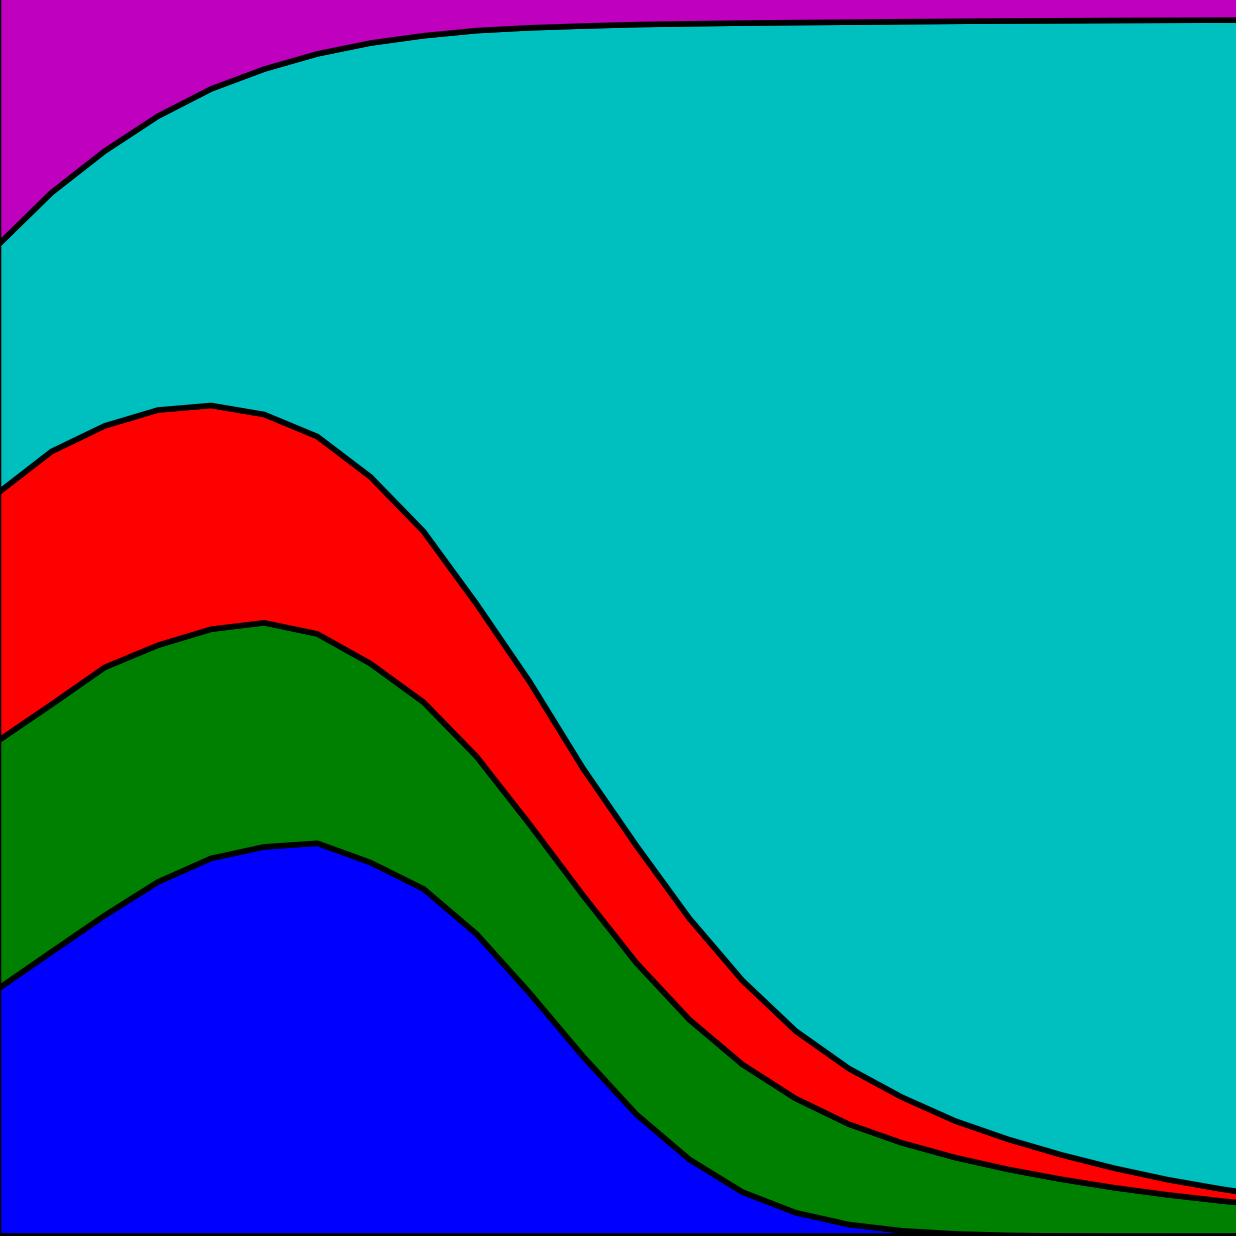
\includegraphics[width=0.24\textwidth]{static/axelrod-logo.png}

    \end{center}
\end{frame}

\begin{frame}
    \begin{center}
    \Large
    \textcolor{orange}{\textsc{Classical Game Theory}} \\ \vspace{3pt}
    \includegraphics[width=0.07\textwidth]{static/Classical.png} \\ \vspace{20pt}

    \textcolor{orange}{\textsc{Evolutionary Game Theory}} \\ \vspace{3pt}
    
\includegraphics[width=0.07\textwidth]{static/evolution.png}
    \end{center}
\end{frame}

\begin{frame}
    \centering
    
\includegraphics[width=.2\textwidth]{static/players} \hspace{.6cm}
    
\includegraphics[width=.2\textwidth]{static/actions} \hspace{.6cm}
    
\includegraphics[width=.2\textwidth]{static/objective}
\end{frame}

\begin{frame}
    \begin{center}
    \includestandalone[width=.75\textwidth]{static/rock_paper_scissors_one}
    \end{center}
\end{frame}

\begin{frame}
    \begin{center}
    \includestandalone[width=.75\textwidth]{static/rock_paper_scissors_two}
    \end{center}
\end{frame}

\begin{frame}
    \begin{center}
    \includestandalone[width=.75\textwidth]{static/rock_paper_scissors_three}
    \end{center}
\end{frame}

\begin{frame}
    \centering
    
\includegraphics[width=.2\textwidth]{static/hawk} 
\includegraphics[width=.2\textwidth]{static/dove}
\end{frame}

\begin{frame}
    \begin{center}
    \LARGE{
        \begin{equation*}
            \begin{pmatrix}
                (0, 0) & (3, 1)  \\
                (1, 3) & (2, 2)
            \end{pmatrix}
        \end{equation*}}
    \end{center}
\end{frame}

\begin{frame}
    \centering
    \includestandalone[width=\textwidth]{static/iterated_hawk_dove}
\end{frame}

\begin{frame}
    \begin{center}
    \includestandalone[width=.55\textwidth]{static/game}
    \end{center}
\end{frame}

% \begin{frame}
%     \begin{center}
%     \includestandalone[width=.55\textwidth]{static/tournament}
%     \end{center}
% \end{frame}

\begin{frame}
    \centering
    
\includegraphics[width=.75\textwidth]{static/Thesis}
\end{frame}

\begin{frame}
    \centering
    
\includegraphics[width=.35\textwidth]{static/evolution.png}
\end{frame}


\begin{frame}
    \begin{center}
    \includestandalone[width=.5\textwidth]{static/evolution}
    \end{center}
\end{frame}

\begin{frame}
    \begin{center}
    \vspace{-1cm}

    \includestandalone[width=.5\textwidth]{static/evolution_two}
    \end{center}
\end{frame}

\begin{frame}
    \begin{center}
        \Large
        \textcolor{orange}{\textsc{Replicator Dynamics}}
    \end{center}
\end{frame}

\begin{frame}
    \begin{columns}
        \begin{column}{.5\textwidth}
            \includestandalone[width=\textwidth]{static/evolution}
        \end{column}
        \begin{column}{.5\textwidth}
            \begin{align*}
                \chi & = (x_1, x_2)
            \end{align*}
            \begin{align*}
                f_1(\chi) & = 0 \times x_1 + 3 \times x_2 \\
                f_2(\chi) & = 1 \times x_1 + 2 \times x_2 \\
            \end{align*}
            \begin{align*}
                \phi & = x_1 f_1(\chi) + x_2 f_2(\chi) \\
                \frac{dx_1}{dt} & = x_1(f_1(\chi) - \phi) 
        \end{align*}
        \end{column}
    \end{columns}
\end{frame}

\begin{frame}
    \begin{center}
    \includestandalone[width=.8\textwidth]{static/phase}
    \end{center}
\end{frame}

\begin{frame}
    \begin{center}
        \Large
        \textcolor{orange}{\textsc{Moran Proccess}} \\ \vspace{3pt}
    \end{center}
\end{frame}

\begin{frame}
    \begin{center}
    \includestandalone[width=\textwidth]{static/moran}
    \end{center}
\end{frame}

\begin{frame}
    \begin{columns}
        \begin{column}{.5\textwidth}
            \includestandalone[width=.8\textwidth]{static/explanation}
        \end{column}
        \begin{column}{.5\textwidth}
            \begin{align*}
                f_{1i} & = \frac{0 \times (i - 1) + 3 \times (N - i)} {N - 1} \\
                f_{2i} & = \frac{1 \times i + 2 \times (N - i - 1)} {N - 1}
            \end{align*}
            \begin{align*}
                p_{i, i + 1} & = \frac{i f_{1i}} {i f_{1i} + (N - i) f_{2i}} \frac{N - i}{N}\\
                p_{i, i - 1} & = \frac{(N - i) f_{2i}} {i f_{1i} + (N - i) f_{2i}} \frac{i}{N}
            \end{align*}
            \begin{align*}
            \varphi = \frac{1}{1+\sum_{i=1}^{N-1}\prod_k^i \frac{p_{i, i - 1}}{p_{i, i + 1}}}.
        \end{align*}
        \end{column}
    \end{columns}
\end{frame}

\begin{frame}
    \begin{center}
        \Large
        \textcolor{orange}{\textsc{Evolution of Cooperation?}}
    \end{center}
\end{frame}


\begin{frame}
    \begin{center}
        \Large
        \textcolor{orange}{\textsc{Prisoner's Dilemma}}
    \end{center}
\end{frame}

\begin{frame}
    \begin{center}
    \LARGE{
        \begin{equation*}
            \begin{pmatrix}
                (1, 1) & (5, 0)  \\
                (5, 0) & (1, 1)
            \end{pmatrix}
        \end{equation*}}
    \end{center}
\end{frame}

\begin{frame}
    \begin{center}
        \Large
        \textcolor{orange}{\textsc{Group Dynamics of Social Behaviour}}
    \end{center}
\end{frame}

\begin{frame}
    \begin{center}
        \Large
        \textcolor{orange}{\textsc{Moran Proccess}} \\ \vspace{3pt}
    \end{center}
\end{frame}

\begin{frame}
    \centering
    
\includegraphics[width=.75\textwidth]{static/close.png}
\end{frame}

\begin{frame}
    \begin{center}
    \faTwitter @NikoletaGlyn \\
    http://web.evolbio.mpg.de/social-behaviour/
    \end{center}
\end{frame}

\end{document}

